% Options for packages loaded elsewhere
\PassOptionsToPackage{unicode}{hyperref}
\PassOptionsToPackage{hyphens}{url}
%
\documentclass[
]{article}
\author{}
\date{}

\usepackage{amsmath,amssymb}
\usepackage{lmodern}
\usepackage{iftex}
\ifPDFTeX
  \usepackage[T1]{fontenc}
  \usepackage[utf8]{inputenc}
  \usepackage{textcomp} % provide euro and other symbols
\else % if luatex or xetex
  \usepackage{unicode-math}
  \defaultfontfeatures{Scale=MatchLowercase}
  \defaultfontfeatures[\rmfamily]{Ligatures=TeX,Scale=1}
  \setmainfont[]{DejaVu Sans}
  \setmonofont[]{DejaVu Sans Mono}
\fi
% Use upquote if available, for straight quotes in verbatim environments
\IfFileExists{upquote.sty}{\usepackage{upquote}}{}
\IfFileExists{microtype.sty}{% use microtype if available
  \usepackage[]{microtype}
  \UseMicrotypeSet[protrusion]{basicmath} % disable protrusion for tt fonts
}{}
\makeatletter
\@ifundefined{KOMAClassName}{% if non-KOMA class
  \IfFileExists{parskip.sty}{%
    \usepackage{parskip}
  }{% else
    \setlength{\parindent}{0pt}
    \setlength{\parskip}{6pt plus 2pt minus 1pt}}
}{% if KOMA class
  \KOMAoptions{parskip=half}}
\makeatother
\usepackage{xcolor}
\IfFileExists{xurl.sty}{\usepackage{xurl}}{} % add URL line breaks if available
\IfFileExists{bookmark.sty}{\usepackage{bookmark}}{\usepackage{hyperref}}
\hypersetup{
  hidelinks,
  pdfcreator={LaTeX via pandoc}}
\urlstyle{same} % disable monospaced font for URLs
\usepackage[a4paper,margin=2cm]{geometry}
\usepackage{color}
\usepackage{fancyvrb}
\newcommand{\VerbBar}{|}
\newcommand{\VERB}{\Verb[commandchars=\\\{\}]}
\DefineVerbatimEnvironment{Highlighting}{Verbatim}{commandchars=\\\{\}}
% Add ',fontsize=\small' for more characters per line
\newenvironment{Shaded}{}{}
\newcommand{\AlertTok}[1]{\textcolor[rgb]{1.00,0.00,0.00}{\textbf{#1}}}
\newcommand{\AnnotationTok}[1]{\textcolor[rgb]{0.38,0.63,0.69}{\textbf{\textit{#1}}}}
\newcommand{\AttributeTok}[1]{\textcolor[rgb]{0.49,0.56,0.16}{#1}}
\newcommand{\BaseNTok}[1]{\textcolor[rgb]{0.25,0.63,0.44}{#1}}
\newcommand{\BuiltInTok}[1]{#1}
\newcommand{\CharTok}[1]{\textcolor[rgb]{0.25,0.44,0.63}{#1}}
\newcommand{\CommentTok}[1]{\textcolor[rgb]{0.38,0.63,0.69}{\textit{#1}}}
\newcommand{\CommentVarTok}[1]{\textcolor[rgb]{0.38,0.63,0.69}{\textbf{\textit{#1}}}}
\newcommand{\ConstantTok}[1]{\textcolor[rgb]{0.53,0.00,0.00}{#1}}
\newcommand{\ControlFlowTok}[1]{\textcolor[rgb]{0.00,0.44,0.13}{\textbf{#1}}}
\newcommand{\DataTypeTok}[1]{\textcolor[rgb]{0.56,0.13,0.00}{#1}}
\newcommand{\DecValTok}[1]{\textcolor[rgb]{0.25,0.63,0.44}{#1}}
\newcommand{\DocumentationTok}[1]{\textcolor[rgb]{0.73,0.13,0.13}{\textit{#1}}}
\newcommand{\ErrorTok}[1]{\textcolor[rgb]{1.00,0.00,0.00}{\textbf{#1}}}
\newcommand{\ExtensionTok}[1]{#1}
\newcommand{\FloatTok}[1]{\textcolor[rgb]{0.25,0.63,0.44}{#1}}
\newcommand{\FunctionTok}[1]{\textcolor[rgb]{0.02,0.16,0.49}{#1}}
\newcommand{\ImportTok}[1]{#1}
\newcommand{\InformationTok}[1]{\textcolor[rgb]{0.38,0.63,0.69}{\textbf{\textit{#1}}}}
\newcommand{\KeywordTok}[1]{\textcolor[rgb]{0.00,0.44,0.13}{\textbf{#1}}}
\newcommand{\NormalTok}[1]{#1}
\newcommand{\OperatorTok}[1]{\textcolor[rgb]{0.40,0.40,0.40}{#1}}
\newcommand{\OtherTok}[1]{\textcolor[rgb]{0.00,0.44,0.13}{#1}}
\newcommand{\PreprocessorTok}[1]{\textcolor[rgb]{0.74,0.48,0.00}{#1}}
\newcommand{\RegionMarkerTok}[1]{#1}
\newcommand{\SpecialCharTok}[1]{\textcolor[rgb]{0.25,0.44,0.63}{#1}}
\newcommand{\SpecialStringTok}[1]{\textcolor[rgb]{0.73,0.40,0.53}{#1}}
\newcommand{\StringTok}[1]{\textcolor[rgb]{0.25,0.44,0.63}{#1}}
\newcommand{\VariableTok}[1]{\textcolor[rgb]{0.10,0.09,0.49}{#1}}
\newcommand{\VerbatimStringTok}[1]{\textcolor[rgb]{0.25,0.44,0.63}{#1}}
\newcommand{\WarningTok}[1]{\textcolor[rgb]{0.38,0.63,0.69}{\textbf{\textit{#1}}}}
\usepackage{graphicx}
\makeatletter
\def\maxwidth{\ifdim\Gin@nat@width>\linewidth\linewidth\else\Gin@nat@width\fi}
\def\maxheight{\ifdim\Gin@nat@height>\textheight\textheight\else\Gin@nat@height\fi}
\makeatother
% Scale images if necessary, so that they will not overflow the page
% margins by default, and it is still possible to overwrite the defaults
% using explicit options in \includegraphics[width, height, ...]{}
\setkeys{Gin}{width=\maxwidth,height=\maxheight,keepaspectratio}
% Set default figure placement to htbp
\makeatletter
\def\fps@figure{htbp}
\makeatother
\setlength{\emergencystretch}{3em} % prevent overfull lines
\providecommand{\tightlist}{%
  \setlength{\itemsep}{0pt}\setlength{\parskip}{0pt}}
\setcounter{secnumdepth}{-\maxdimen} % remove section numbering
% Make \paragraph and \subparagraph free-standing
\ifx\paragraph\undefined\else
  \let\oldparagraph\paragraph
  \renewcommand{\paragraph}[1]{\oldparagraph{#1}\mbox{}}
\fi
\ifx\subparagraph\undefined\else
  \let\oldsubparagraph\subparagraph
  \renewcommand{\subparagraph}[1]{\oldsubparagraph{#1}\mbox{}}
\fi
\usepackage{fancyhdr}
\pagestyle{fancy}
\lhead{}
\chead{md2pdf}
\rhead{}
\ifLuaTeX
  \usepackage{selnolig}  % disable illegal ligatures
\fi

\begin{document}

\hypertarget{md2pdf}{%
\section{md2pdf}\label{md2pdf}}

A small script to convert markdown to pdf using pandoc with custom
settings

\hypertarget{dependencies}{%
\subsection{Dependencies}\label{dependencies}}

\hypertarget{arch-based-distributions}{%
\subsubsection{Arch based
Distributions}\label{arch-based-distributions}}

\begin{Shaded}
\begin{Highlighting}[]
\FunctionTok{sudo}\NormalTok{ pacman }\AttributeTok{{-}S}\NormalTok{ pandoc ttf{-}dejavu texlive{-}core}
\end{Highlighting}
\end{Shaded}

\hypertarget{debian-based-distributions}{%
\subsubsection{Debian based
Distributions}\label{debian-based-distributions}}

\begin{Shaded}
\begin{Highlighting}[]
\FunctionTok{sudo}\NormalTok{ apt install pandoc fonts{-}dejavu texlive{-}xetex}
\end{Highlighting}
\end{Shaded}

\hypertarget{other}{%
\subsubsection{Other}\label{other}}

You can probably figure it out yourself, based on the two commands above

\hypertarget{manual-installation}{%
\subsection{Manual Installation}\label{manual-installation}}

\begin{enumerate}
\def\labelenumi{\arabic{enumi}.}
\tightlist
\item
  Download the
  \href{https://raw.githubusercontent.com/RubixDev/md2pdf/main/md2pdf.sh}{md2pdf}
  file:\\
  \texttt{wget\ https://raw.githubusercontent.com/RubixDev/md2pdf/main/md2pdf.sh}
\item
  Replace `YOUR NAME HERE' at the top with your actual name. This will
  appear in the header of the exported PDFs:\\
  \texttt{sed\ -i\ \textquotesingle{}s/YOUR\ NAME\ HERE/\textless{}name\textgreater{}/g\textquotesingle{}\ md2pdf.sh}
\item
  Rename it to \texttt{md2pdf} without \texttt{.sh}:\\
  \texttt{mv\ md2pdf.sh\ md2pdf}
\item
  Make the file executable:\\
  \texttt{chmod\ +x\ md2pdf}
\item
  Move the file to \texttt{/usr/local/bin}\\
  \texttt{sudo\ mv\ md2pdf\ /usr/local/bin/}
\end{enumerate}

\hypertarget{automatic-installation}{%
\subsection{Automatic Installation}\label{automatic-installation}}

Alternatively, you can also use the automatic install script, which asks
for your name (which will appear in the header of the PDFs) and places
the file in \texttt{/usr/local/bin}, which should be in your PATH.

\hypertarget{for-fish-users}{%
\subsubsection{For fish users:}\label{for-fish-users}}

\begin{Shaded}
\begin{Highlighting}[]
\FunctionTok{wget}\NormalTok{ https://raw.githubusercontent.com/RubixDev/md2pdf/main/install.sh}
\FunctionTok{bash}\NormalTok{ install.sh}
\FunctionTok{rm}\NormalTok{ install.sh}
\end{Highlighting}
\end{Shaded}

\hypertarget{for-the-rest}{%
\subsubsection{For the rest:}\label{for-the-rest}}

\begin{Shaded}
\begin{Highlighting}[]
\FunctionTok{bash} \AttributeTok{{-}c} \StringTok{"}\VariableTok{$(}\ExtensionTok{curl} \AttributeTok{{-}fsSL}\NormalTok{ https://raw.githubusercontent.com/RubixDev/md2pdf/main/install.sh}\VariableTok{)}\StringTok{"}
\end{Highlighting}
\end{Shaded}

or

\begin{Shaded}
\begin{Highlighting}[]
\FunctionTok{bash} \AttributeTok{{-}c} \StringTok{"}\VariableTok{$(}\FunctionTok{wget} \AttributeTok{{-}O{-}}\NormalTok{ https://raw.githubusercontent.com/RubixDev/md2pdf/main/install.sh}\VariableTok{)}\StringTok{"}
\end{Highlighting}
\end{Shaded}

\hypertarget{usage}{%
\subsection{Usage}\label{usage}}

\begin{Shaded}
\begin{Highlighting}[]
\ExtensionTok{md2pdf} \OperatorTok{\textless{}}\NormalTok{input file}\OperatorTok{\textgreater{}} \OperatorTok{\textless{}}\NormalTok{output file}\OperatorTok{\textgreater{}} \DataTypeTok{\textbackslash{}}
    \AttributeTok{{-}l}\KeywordTok{|}\ExtensionTok{{-}{-}left{-}head}\NormalTok{ [header left text] }\DataTypeTok{\textbackslash{}}
    \AttributeTok{{-}c}\KeywordTok{|}\ExtensionTok{{-}{-}center{-}head}\NormalTok{ [header center text] }\DataTypeTok{\textbackslash{}}
    \AttributeTok{{-}r}\KeywordTok{|}\ExtensionTok{{-}{-}right{-}head}\NormalTok{ [header right text] }\DataTypeTok{\textbackslash{}}
    \AttributeTok{{-}n}\KeywordTok{|}\ExtensionTok{{-}{-}name{-}location}\NormalTok{ [left}\KeywordTok{|}\ExtensionTok{center}\KeywordTok{|}\ExtensionTok{right]} \DataTypeTok{\textbackslash{}}
    \AttributeTok{{-}{-}preserve{-}tex}
\end{Highlighting}
\end{Shaded}

\begin{itemize}
\tightlist
\item
  \texttt{-l}, \texttt{-c}, \texttt{-r} and their long counterparts
  control the text to appear in the head of each page
\item
  \texttt{-n} or \texttt{-\/-name-location} followed by one of
  \texttt{left}, \texttt{center} or \texttt{right} controls where to
  place the name in the head

  \begin{itemize}
  \tightlist
  \item
    By default it will be placed left
  \item
    The name can be overwritten by the previously mentioned flags
  \item
    If anything else is provided, the name will not be displayed
  \end{itemize}
\item
  The \texttt{-\/-preserve-tex} option keeps the generated \texttt{.tex}
  file
\end{itemize}

\hypertarget{examples}{%
\subsubsection{Examples}\label{examples}}

\begin{Shaded}
\begin{Highlighting}[]
\ExtensionTok{md2pdf}\NormalTok{ README.md README.pdf}
\end{Highlighting}
\end{Shaded}


\includegraphics{Images/Example1.png}

\begin{Shaded}
\begin{Highlighting}[]
\ExtensionTok{md2pdf}\NormalTok{ README.md README.pdf }\AttributeTok{{-}l} \StringTok{" "}
\end{Highlighting}
\end{Shaded}


\includegraphics{Images/Example2.png}

\begin{Shaded}
\begin{Highlighting}[]
\ExtensionTok{md2pdf}\NormalTok{ README.md README.pdf }\AttributeTok{{-}l}\NormalTok{ 29.08.2021 }\AttributeTok{{-}n}\NormalTok{ right}
\end{Highlighting}
\end{Shaded}


\includegraphics{Images/Example3.png}

\begin{Shaded}
\begin{Highlighting}[]
\ExtensionTok{md2pdf}\NormalTok{ README.md README.pdf }\DataTypeTok{\textbackslash{}}
    \AttributeTok{{-}{-}center{-}head} \StringTok{"Text with spaces"} \DataTypeTok{\textbackslash{}}
    \AttributeTok{{-}{-}right{-}head}\NormalTok{ 29.08.2021 }\DataTypeTok{\textbackslash{}}
    \AttributeTok{{-}{-}name{-}location}\NormalTok{ left}
\end{Highlighting}
\end{Shaded}

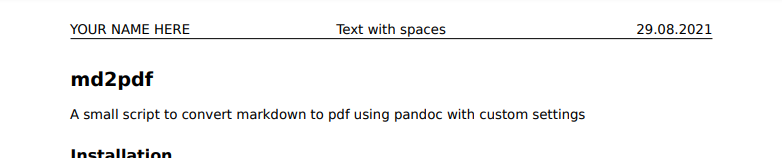
\includegraphics{Images/Example4.png}

\end{document}
